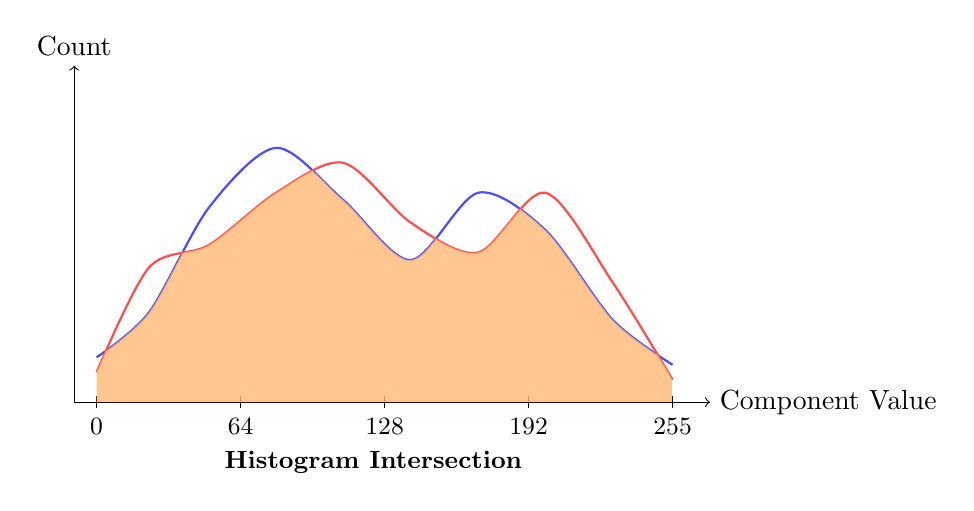
\begin{tikzpicture}[scale=0.95]
    % Axes
    \draw[->] (0,0) -- (8.5,0) node[right] {Component Value};
    \draw[->] (0,0) -- (0,4.5) node[above] {Count};

    % X-axis ticks (0--255 scale)
    \foreach \x/\label in {
        0.3/0,
        2.225/64,
        4.15/128,
        6.075/192,
        8/255
    }{
        \draw (\x,0.08) -- (\x,-0.08);
        \node[below] at (\x,-0.08) {\small \label};
    }

    % Blue histogram curve
    \draw[blue!70, thick]
    plot[smooth]
    coordinates {
    (0.3,0.6) (1,1.2) (1.8,2.6)
    (2.7,3.4) (3.6,2.7) (4.5,1.9)
    (5.4,2.8) (6.3,2.3) (7.2,1.1)
    (8,0.5)
    };

    % Red histogram curve
    \draw[red!70, thick]
    plot[smooth]
    coordinates {
    (0.3,0.4) (1,1.8) (1.8,2.1)
    (2.7,2.8) (3.6,3.2) (4.5,2.4)
    (5.4,2.0) (6.3,2.8) (7.2,1.6)
    (8,0.3)
    };

    % Intersection fill
    \begin{scope}
    \clip
    plot[smooth]
    coordinates {
    (0.3,0.6) (1,1.2) (1.8,2.6)
    (2.7,3.4) (3.6,2.7) (4.5,1.9)
    (5.4,2.8) (6.3,2.3) (7.2,1.1)
    (8,0.5)
    }
    -- (8,0) -- (0.3,0) -- cycle;

    \fill[orange!55, opacity=0.8]
    plot[smooth]
    coordinates {
    (0.3,0.4) (1,1.8) (1.8,2.1)
    (2.7,2.8) (3.6,3.2) (4.5,2.4)
    (5.4,2.0) (6.3,2.8) (7.2,1.6)
    (8,0.3)
    }
    -- (8,0) -- (0.3,0) -- cycle;
    \end{scope}

    % Caption
    \node[font=\small] at (4,-0.8)
    {\textbf{Histogram Intersection}};
\end{tikzpicture}